\documentclass[tikz,border=2pt]{standalone}
\usepackage{amsmath,amssymb}
\usepackage{tikz}
\usetikzlibrary{arrows.meta}

\begin{document}
% Three faces of continuity: convergent sequences are sent to convergent sequences, and the
% preimage of an open set V is open.
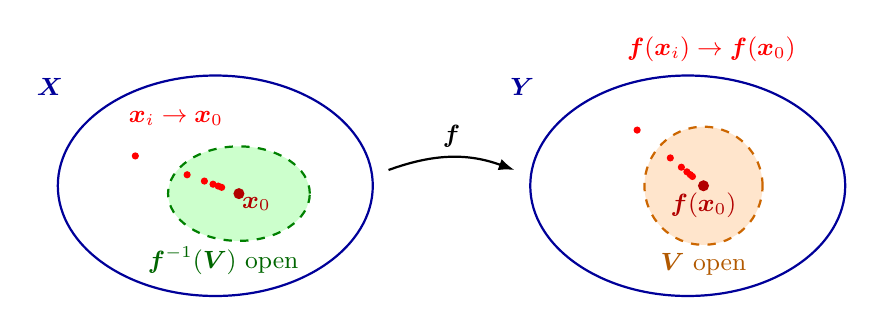
\begin{tikzpicture}[every node/.style={font=\small}, >={Latex[length=2mm]}]
	\draw[thick, blue!60!black] (0,0) ellipse (2 and 1.4);
	\node[blue!60!black] at (-2.1,1.25) {$\boldsymbol{X}$};
	\fill[green!20] (0.3,-0.1) ellipse (0.9 and 0.6);
	\draw[green!50!black, dashed, thick] (0.3,-0.1) ellipse (0.9 and 0.6);
	\node[green!40!black, font=\small] at (0.1,-0.95) {$\boldsymbol{f}^{-1}(\boldsymbol{V})$ open};
	\foreach \i in {1,...,6} {\fill[red] ({0.3-1.4/\i*cos(20)}, {-0.1+1.4/\i*sin(20)}) circle (1.3pt);}
	\fill[red!70!black] (0.3,-0.1) circle (2pt);
	\node[red!70!black, below right, inner sep=1pt] at (0.3,-0.1) {$\boldsymbol{x}_0$};
	\node[red, font=\small] at (-0.5,0.85) {$\boldsymbol{x}_i\to\boldsymbol{x}_0$};
	\draw[->, thick] (2.2,0.2) to[bend left=20] node[above] {$\boldsymbol{f}$} (3.8,0.2);
	\begin{scope}[xshift=6cm]
		\draw[thick, blue!60!black] (0,0) ellipse (2 and 1.4);
		\node[blue!60!black] at (-2.1,1.25) {$\boldsymbol{Y}$};
		\fill[orange!20] (0.2,0) circle (0.75);
		\draw[orange!80!black, dashed, thick] (0.2,0) circle (0.75);
		\node[orange!70!black, font=\small] at (0.2,-1.0) {$\boldsymbol{V}$ open};
		\foreach \i in {1,...,6} {\fill[red] ({0.2+1.1/\i*cos(140)}, {1.1/\i*sin(140)}) circle (1.3pt);}
		\fill[red!70!black] (0.2,0) circle (2pt);
		\node[red!70!black, below, inner sep=2.5pt] at (0.2,0) {$\boldsymbol{f}(\boldsymbol{x}_0)$};
		\node[red, font=\small, anchor=south] at (0.3,1.45) {$\boldsymbol{f}(\boldsymbol{x}_i)\to\boldsymbol{f}(\boldsymbol{x}_0)$};
	\end{scope}
\end{tikzpicture}
\end{document}
